%%%%%%%%%%%%%%%%%%%%%
% Documento maestro %
%%%%%%%%%%%%%%%%%%%%%
\documentclass{fime}

%%%%%%%%%%%%%%%%%%%%%%%%%%%%%%%%%%%%%%%%%%%
% Cargando paquetes y definiendo opciones %
%%%%%%%%%%%%%%%%%%%%%%%%%%%%%%%%%%%%%%%%%%%
% Aquí puedes cargar los paquetes que vas a usar. La clase
% fime ya incluye babel, inputenc, graphicx y los de la AMS.
% C1argar un paquete está a tu libertad (y responsabilidad).
\usepackage{hyperref}
\usepackage{graphicx}
\usepackage{subfig}
\usepackage{pdflscape}
\usepackage[numbers,sort&compress]{natbib}
\usepackage{float}
\usepackage{footmisc}
\usepackage{adjustbox}
\usepackage{tikz}
\usepackage{listing}
\usepackage{pythonhighlight}
\usepackage{rotating}
\usepackage{array,booktabs,makecell}
\usetikzlibrary{arrows, babel, shapes}
\usepackage[font=small, skip=0pt]{caption}
\setlength{\footnotesep}{0.5cm}
\setlength\footnotemargin{3pt}
\hypersetup{breaklinks=true,colorlinks=true,    linkcolor=black,citecolor=black,urlcolor=black}
\usepackage[nodisplayskipstretch]{setspace}
\setstretch{1.5}
\tikzstyle{decision} = [diamond, draw, fill=yellow!20, text width=8em, text badly centered, node distance=3.5cm, inner sep=0pt]
\tikzstyle{block} = [rectangle, draw, fill=blue!20, text width=12em, text centered, rounded corners, minimum height=4em]
\tikzstyle{line} = [draw, -latex']
\tikzstyle{cloud} = [draw, ellipse,fill=red!20, node distance=1cm,minimum height=4em, text width=4em, text centered]

\renewcommand{\lstlistingname}{Código}
\renewcommand{\lstlistlistingname}{Lista de \lstlistingname s}
%%%%%%%%%%%%%%%%%%%%%
% Definiendo campos %
%%%%%%%%%%%%%%%%%%%%%
\def\titulo{Modelado y visualización de relaciones entre contaminantes de aire y salud pública}
\def\autor{Selene Berenice Prado Prado}
\def\matricula{1810042}
\def\grado{Ingeniería en Tecnología de Software}
% En caso de que el grado tenga orientación o especialidad llenar el siguiente
% campo dejando un ESPACIO INICIAL, en caso contrario, dejar vacío
\def\orientacion{}
\def\fecha{Enero 2022} % Coloca el mes con mayúscula inicial

\def\asesor{Dra. Satu Elisa Schaeffer}
\def\revisorA{Dra. Sara Elena Garza Villarreal}
\def\revisorB{Dra. Sara Verónica Rodríguez Sánchez}
% En el caso de que tu tesis sea de doctorado activa la variable cambiándola a \doctoradotrue
% y define tus otros dos revisores
\newif\ifdoctorado\doctoradofalse
\def\revisorC{Nombre del revisor C}
\def\revisorD{Nombre del revisor D}
% El visto bueno siempre va
\def\vobo{Dr. Fernando Banda Muñoz}

%%%%%%%%%%%%%%%%%%%%%%%
% Inicia el documento %
%%%%%%%%%%%%%%%%%%%%%%%
\begin{document}

\frontmatter
\pagestyle{main}

%%% Incluye PortillasM si tu tesis es de Maestría
%%% y PortillasD si es de doctorado.
% Portadas (Maestría)

\def\uanl{Universidad Autónoma de Nuevo León}
\def\fime{Facultad de Ingeniería Mecánica y Eléctrica}
\def\depg{Subdirección Académica}
\def\snnl{San Nicolás de los Garza, Nuevo León}

%%%%%%%%%%%%%%%%%%%%%%%%
% Primer portada: UANL %
%%%%%%%%%%%%%%%%%%%%%%%%
\thispagestyle{empty}

\begin{scshape}
\begin{center}
	{\Large \uanl} \\[5mm]
	{\large \fime} \\[5mm]
	{\large \depg}
	\vskip 15mm
	
\includegraphics[height=55mm]{uanl}
	\vskip 12mm
	\begin{tabular}{p{11cm}}
		\centering
		{\large \titulo}
	\end{tabular}
	\vskip 7mm
	{por}\\[7mm]
	{\large \autor}\\[7mm]
	{como requisito parcial para obtener el grado de}\\[3mm]
	\MakeUppercase{\grado}\\
	\orientacion
	\vfill
	\fecha
\end{center}
\end{scshape}

%%%%%%%%%%%%%%%%%%%%%%%%%
% Segunda portada: FIME %
%%%%%%%%%%%%%%%%%%%%%%%%%
\newpage
\thispagestyle{empty}

\begin{scshape}
\begin{center}
	{\Large \uanl} \\[5mm]
	{\large \fime} \\[5mm]
	{\large \depg}
	\vskip 16mm
	
\includegraphics[height=50mm]{fime}
	\vskip 16mm
	\begin{tabular}{p{11cm}}
		\centering
		{\large \titulo}
	\end{tabular}
	\vskip 7mm
	{por}\\[7mm]
	{\large \autor}\\[7mm]
	{como requisito parcial para obtener el grado de}\\[3mm]
	\MakeUppercase{\grado}\\
	\orientacion
	\vfill
	\fecha
\end{center}
\end{scshape}

%%%%%%%%%%%%%%%%%%%%%%%%%%%%%
% Carta del comité de tesis %
%%%%%%%%%%%%%%%%%%%%%%%%%%%%%
\newpage
\thispagestyle{empty}
\enlargethispage{5mm}

\begin{center}
{\bf \large \uanl} \\
{\bf \fime} \\
{\bf \depg}
\end{center}
\vskip 4mm

Los miembros del Comité de Tesis recomendamos que la Tesis <<\titulo>>, realizada por el alumno \autor, con número de matrícula \matricula, sea aceptada para su defensa como requisito parcial para obtener el grado de \grado\orientacion.
\ifdoctorado{\vskip 10mm}\else{\vskip 8mm}\fi

\begin{center}
El Comité de Tesis\\
\ifdoctorado{\vskip 15mm}\else{\vskip 25mm}\fi

\ifdoctorado{%%%
\begin{tabular}{p{37mm}p{21mm}p{12mm}p{21mm}p{37mm}}
	\cline{2-4}
	& \multicolumn{3}{c}{\asesor} & \\
	& \multicolumn{3}{c}{Asesor}  & \\[15mm]
	\cline{1-2} \cline{4-5}
	\multicolumn{2}{c}{\revisorA} & & \multicolumn{2}{c}{\revisorB} \\
	\multicolumn{2}{c}{Revisor}   & & \multicolumn{2}{c}{Revisor}   \\[17mm]
	\cline{1-2} \cline{4-5}
	\multicolumn{2}{c}{\revisorC} & & \multicolumn{2}{c}{\revisorD} \\
	\multicolumn{2}{c}{Revisor}   & & \multicolumn{2}{c}{Revisor}   \\[2mm]
	& \multicolumn{3}{c}{Vo. Bo.} & \\[14mm]
	\cline{2-4}
	& \multicolumn{3}{c}{\vobo}   & \\
	& \multicolumn{3}{c}{\depg}   & \\ &&&&
\end{tabular}
}\else{%%%
\begin{tabular}{p{37mm}p{21mm}p{12mm}p{21mm}p{37mm}}
	\cline{2-4}
	& \multicolumn{3}{c}{\asesor} & \\
	& \multicolumn{3}{c}{Asesora}  & \\[19mm]
	\cline{1-2} \cline{4-5}
	\multicolumn{2}{c}{\revisorA} & & \multicolumn{2}{c}{\revisorB} \\
	\multicolumn{2}{c}{Revisora}   & & \multicolumn{2}{c}{Revisora}   \\[2mm]
	& \multicolumn{3}{c}{Vo. Bo.} & \\[17mm]
	\cline{2-4}
	& \multicolumn{3}{c}{\vobo}   & \\
	& \multicolumn{3}{c}{\depg}   & \\ &&&&
\end{tabular}
}\fi%%%

\vfill

\snnl, \MakeLowercase{\fecha}

\end{center}

%%%% Dedicatoria

\thispagestyle{empty}
\vspace*{17mm}

\begin{flushright}
\begin{itshape}

Aquí puedes poner tu dedicatoria\\
si es que tienes una.\bigskip\bigskip

Si no tienes una, puedes borrar\\
la línea \verb+% Dedicatoria

\thispagestyle{empty}
\vspace*{17mm}

\begin{flushright}
\begin{itshape}

Aquí puedes poner tu dedicatoria\\
si es que tienes una.\bigskip\bigskip

Si no tienes una, puedes borrar\\
la línea \verb+% Dedicatoria

\thispagestyle{empty}
\vspace*{17mm}

\begin{flushright}
\begin{itshape}

Aquí puedes poner tu dedicatoria\\
si es que tienes una.\bigskip\bigskip

Si no tienes una, puedes borrar\\
la línea \verb+\include{Dedicatoria}+ en el\\
archivo \texttt{MiTesis.tex} pues no es obligatoria.

\end{itshape}
\end{flushright}

+ en el\\
archivo \texttt{MiTesis.tex} pues no es obligatoria.

\end{itshape}
\end{flushright}

+ en el\\
archivo \texttt{MiTesis.tex} pues no es obligatoria.

\end{itshape}
\end{flushright}



\tableofcontents
\listoffigures
\listoftables

%Agradecimientos

\chapter{Agradecimientos}
\markboth{Agradecimientos}{}

Quiero agradecer a la Dra. Elisa, por el apoyo, el conocimiento y el tiempo que invirtió durante el desarrollo de mi tesis para poder hacer una gran investigación. Al Dr. Manuel Jiménez, por el material brindado además de los aportes que hizo para complementar la tesis y al Fondo Sectorial de Investigación Ambiental SEMARNAT-CONACYT con No. de proyecto 263080.

A mis padres, José Angel y Bertha Alicia, quienes siempre me motivaron a seguir adelante y son el motor de mi vida. A mis hermanas y sobrinos por su gran apoyo en todo momento, a mis abuelos Sara y José Reyes que siempre me motivaron a crecer como persona y alcanzar la meta de superarme.

Mención especial a mi abuelo Reyes (QEPD), quien en todo momento, incluso meses antes de fallecer, siempre me apoyó y esperó que diera todo de mí para ser alguien mejor de lo que él fue.

%... debo mejorar esto, pero ya sé a quienes debo/quiero agradecer..
%Resumen

\chapter{Resumen}
\markboth{Resumen}{}

{\setlength{\leftskip}{10mm}
\setlength{\parindent}{-10mm}

\autor.

Candidato para obtener el grado de \grado\orientacion.

\uanl.

\fime.

Título del estudio: \textsc{\titulo}.

\noindent Número de páginas: \pageref*{lastpage}.}

%%% Comienza a llenar aquí
\paragraph{Objetivos y método de estudio:}
El objetivo de la investigación es generar modelos que permitan visualizar relaciones entre contaminantes atmosféricos y salud pública. Los modelos generados se utilizan en conjunto con datos obtenidos de la Secretaría de Salud del Gobierno de México y registros de los niveles de los contaminantes presentes en el área metropolitana de Monterrey. 

El tener un modelo que permita visualizar relaciones entre contaminantes atmosféricos y salud pública que sea utilizado con datos confiables y verídicos pueden ayudar a entender el impacto que tiene el aumento del nivel de contaminantes atmosféricos.
\paragraph{Contribuciones y conclusiones:}
En la investigación se exploran diversas maneras de visualizar la información, además de generar modelos que permiten analizar las relaciones existentes entre los niveles de determinados contaminantes y CIE. Las visualizaciones generadas son series de tiempo y gráficos de radar, y modelos de regresión lineal y de regresión lineal múltiple. 

\bigskip\noindent\begin{tabular}{lc}
\vspace*{-2mm}\hspace*{-2mm}Firma de la asesora: & \\
\cline{2-2} & \hspace*{1em}\asesor\hspace*{1em}
\end{tabular}

\bigskip\noindent\begin{tabular}{lc}
\vspace*{-2mm}\hspace*{-2mm}Firma de la coasesora: & \\
\cline{2-2} & \hspace*{1em}\revisorA\hspace*{1em}
\end{tabular}



\mainmatter
\pagestyle{fime}

%%% Haz un documento para cada capítulo
\chapter{Introducción}
El crear modelos para la visualización de datos ayuda a observar con mayor claridad los datos para encontrar relaciones entre ellos.

El \emph{aprendizaje máquina}\footnote{Traducido como \emph{machine learning} en inglés, tiene como objetivo desarrollar técnicas que les permitan a las computadoras aprender.} es un área dentro de la \emph{ciencia de datos}\footnote{Traducido como \emph{data science} en inglés, involucra métodos para extraer conocimiento de datos, eso con la finalidad de que haya un mejor entendimiento de los datos.} que puede ayudar a crear dichos modelos para tener una más eficiente visualización cuando se trabaja con una gran cantidad de datos, que es lo que se requiere para el presente trabajo. El área de la ciencia de datos es muy útil ya que permite trabajar con grandes cantidades de datos aminorando la cantidad de tiempo empleado en la creación de gráficos que permitan visualizar los datos.

La tarea en el presente proyecto es utilizar modelos para visualizar las relaciones entre los contaminantes del aire y salud pública, para ello se requieren datos sobre salud pública y sobre los niveles de contaminantes del aire.

Para la realización de los experimentos se tienen datos de ingresos hospitalarios provenientes de la base de datos de la Secretaría de Salud del Gobierno de México \cite{f1}. También se tienen registros de los niveles de algunos contaminantes del aire presentes en el área metropolitana de Monterrey, dichos registros son hechos por las estaciones de monitoreo pertenecientes al Sistema Integral de Monitoreo Ambiental (SIMA) \cite{f2} mostradas en la figura \ref{estaciones}.

\begin{figure}[h!]
\setcounter{figure}{0} % por culpa de sciposter
\captionsetup{type=figure} % por culpa de sciposter
\begin{center}
   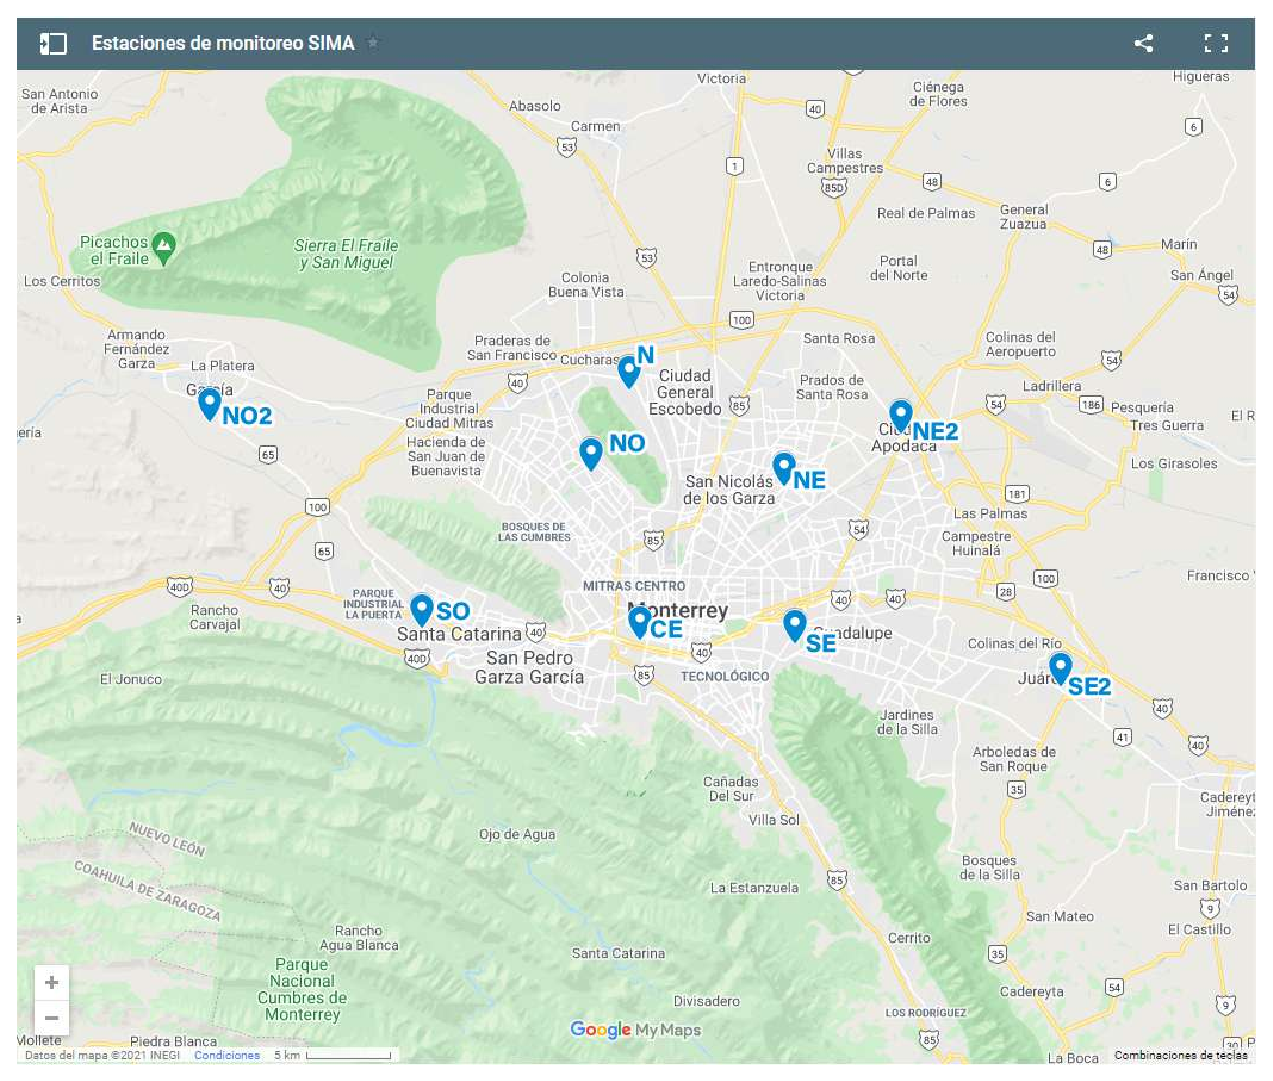
\includegraphics[width=1\textwidth]{mapa_estaciones.eps}
   \end{center}
    \caption{Localización de las estaciones de monitoreo de la calidad del aire.}
    \label{estaciones}
\end{figure}

\clearpage

\section{Motivación}
Existen investigaciones que ya han estudiado las relaciones entre contaminantes del aire y salud pública, sin embargo, con el presente trabajo se busca aportar a la creación de nuevas herramientas que permitan observar y estudiar dichas relaciones. El poder visualizar dichas relaciones puede ayudar a tomar medidas adecuadas que permitan aminorar los efectos negativos de los contaminantes del aire en la salud de las personas.

\section{Hipótesis}
Se plantea que con modelos de regresión se pueden obtener gráficos donde se pueden observar las relaciones entre el número de ingresos hospitalarios y los niveles de contaminantes del aire.

\section{Objetivos}
En esta sección se establece el objetivo general y los objetivos específicos sobre los que se orienta la tesis.

\subsection{Objetivo general}
El objetivo de generar, implementar y evaluar un módelo que muestra las relaciones existentes entre contaminantes del aire y salud pública tiene la finalidad de apoyar a la implementación de estrategías que aminoran los efectos negativos de los contaminantes del aire en la salud de las personas. Con el modelo generado se puede tener una herramienta que permite identificar gráficamente las relaciones con solo proporcionarle el conjunto de datos.

\subsection{Objetivos específicos}
\begin{itemize}
\item Generar, implementar y evaluar un módelo de regresión que permite cuantificar las relaciones entre contaminantes del aire y salud pública a partir de un conjunto de datos.
\end{itemize}
\begin{itemize}
\item Diseñar e implementar visualizaciones interactivas que permiten explorar los modelos implementados y su validez estadística.
\end{itemize}
\begin{itemize}
\item Generar, implementar y evaluar un módelo de regresión que muestra un análisis de datos proporcionados sobre niveles de contaminantes del aire y salud pública.
\end{itemize}
%\begin{itemize}
%\item Generar un módelo de regresión que permite estudiar las relaciones entre los niveles de contaminantes del aire y salud pública.
%\end{itemize}

%\section{Estructura}
%El contenido de la investigación se divide en...


\chapter{Antecedentes}
%En algunos trabajos se han utilizado modelos de series de tiempo y ...

\section{Antecedentes históricos}
\citet{r1} mencionan que uno de los diseños epidemiológicos más utilizados son los estudios de series temporales. Con esos diseños se analizan las variaciones en el tiempo de la exposición al contaminante y el indicador de salud estudiado en una población.

\section{Salud en una comunidad}
Existen factores ambientales que afectan la salud de una comunidad como: el abastecimiento de agua potable y el saneamiento, la vivienda y el hábitat, la alimentación, la contaminación ambiental, el empleo de productos químicos y los riesgos ocupacionales \citep{r2}.

\chapter{Estado del arte}
En este capítulo se explica...

\section{Investigaciones relacionadas}
Existen algunos trabajos que...

\section{Comparación de trabajos}
La mayoría de los trabajos citados...

\subsection{Comparaciones}
En el cuadro...

\subsection{Áreas de oportunidad}
En el cuadro...


\chapter{Solución propuesta}
Habiendo conocido las características que mejor describen a los atributos del presente trabajo, se puede decir que la base del método propuesto se puede desarrollar...

\section{Datos recolectados}
Inicialmente...


\chapter{Desarrollo de la solución}
Recapitulando las fases anteriores, se conoce que...


\chapter{Experimentos}
Después de...

\section{Diseño experimental}
Hola...

\section{Resultados}
Establecidos los experimentos que se van a realizar, se reporta los resultados obtenidos...

\section{Discusión}
Todos los experimentos son ejecutados en una laptop con las especificaciones del cuadro \ref{tab:Especificaciones técnicas del PC}.

\begin{table}[H]
	{\centering
		\caption{Especificaciones técnicas del equipo de cómputo}
		\begin{tabular}{|c|c|c|}
			\hline
			Sistema Operativo & Windows 10 64 bits\\
			\hline
			Procesador & Intel Core i5-7300HQ\\
			\hline
			RAM & 8 GB RAM DDR4 2133 MHz\\
			\hline
		\end{tabular}

	\label{tab:Especificaciones técnicas del PC}
	}
\end{table}


\chapter{Conclusiones}
Este capítulo describe la tesis a partir de la manera que cumple los objetivos generales y específicos para determinar si la hipótesis se comprueba, trata también del porque se realizó la tesis...

\clearpage

\section{Contribuciones}
La solución propuesta surgió a partir de...

\section{Trabajo a futuro}
La solución propuesta en la tesis...

\appendix
%%% Haz un documento para cada apéndice
%%\chapter{CIE y sus nombres de enfermedades}

\begin{table}[H]
	{\centering
		\caption{CIE mencionadas en los Experimentos y el nombre de la enfermedad.}
		\begin{tabular}{|c|c|c|}
			\hline 
			CIE & Enfermedad\\
			\hline
			N40-N53 & Enfermedades de los órganos genitales masculino\\
			\hline
			K00-K93 & Enfermedades del aparato digestivo\\
			\hline
			O00-O99 & Embarazo, parto y puerperio\\
			\hline
		\end{tabular}
		
	\label{tab:CIE y sus nombres de enfermedades}
	}
\end{table}


%En princicpio tienes total libertad de incluir tu bibliografía con el entorno {\tt thebibliography} nativo de \LaTeX{} o mediante la herramienta \textsc{Bib}\TeX. En caso de que optes por esto último (recomendado), puedes usar alguno de los archivos {\tt mighelbib.bst} o {\tt mighelnat.bst} incluidos en el paquete {\tt Tesis-FIME}, pues sus diseños están basados en el estilo bibliográfico estándar del español, además de que armoniza con el estilo de tesis provisto por {\tt fime.cls}.

%El estilo bibliográfico {\tt mighelbib} es numérico, es decir cita con un número entre corchetes, por ejemplo una cita \verb+\cite{Dan82}+ genera una etiqueta del tipo [13], mientras que el estilo {\tt mighelnat} es tipo autor-año y requiere que el paquete {\tt natbib} sea cargado (sin opciones) para su correcto funcionamiento, cita con el apellido del autor y el año, por ejemplo una cita \verb+\citet{Dan82}+ genera una etiqueta del tipo Dantzig (1982), mientras que una cita \verb+\citep{Dan82}+ genera una etiqueta del tipo (Dantzig, 1982).

%Como muestra del estilo, unas citas: un libro clásico de programación lineal \cite{Baz04} y un documento histórico \cite{Dan82}. Para saber un poco más del uso de \textsc{Bib}\TeX, se puede leer \cite{Mat11}.

%\section{Comillas}

%El objetivo de esta sección era provocar otra página para que se vea el encabezado. Pero aprovechamos para decir que la clase {\tt fime.cls} carga el paquete {\tt babel} con la opción {\tt spanish}, por lo que cambiará automáticamente los dobles signos $<<$ y $>>$ por << y >>. Estas comillas angulares son las correctas en el idioma español, y son las que se usan en la clase {\tt fime.cls}, por lo que se sugiere sean las usadas en el texto cada que quieras <<entrecomillar>> algo.



\backmatter
\pagestyle{main}

%%% Aquí va la bibliografía, puedes usar el entorno de LaTeX (thebibliography)
%%% o la herramienta BibTeX. En caso de que optes por BibTeX, puedes usar
%%% alguno de los archivos de estilo (mighelbib.bst o mighelnat.bst) incluidos
%%% en el paquete, cuyos diseños armonizan con el diseño de tesis provisto por
%%% fime.cls. Para muestra, basta un botón:
\bibliographystyle{mighelnat}
\bibliography{MiBiblio}

\label{lastpage}
%Autobiografia

\chapter*{Resumen autobiográfico}
\thispagestyle{empty}

\begin{center}
\autor

Candidato para obtener el grado de\\
\grado\\
\orientacion\bigskip

\uanl\\
\fime\bigskip

Tesis:\\
\textsc{\large\titulo}
\end{center}\bigskip

%Aquí va tu historia
Nací el 30 de Junio de 2000 en Monterrey, Nuevo León, soy la mayor de 4 hijos. Mi familia está conformada por mi madre Lilia Prado López, mi padre Adan Alfaro Lerma, y mis hermanos: Angel Alejandro Prado Prado, Estrella Belen Prado Prado, y Genesis Adali Alfaro Prado. \\
Desde pequeña me han gustado las matemáticas, aprender como funcionan los sistemas computacionales, y leer. \\
Durante los primeros semestres de de mi carrera descubrí la inteligencia computacional, un área que me encantó desde que la descubrí, en especial su rama de ciencia de datos, rama en la que espero seguir desarrollandome. \\
Otra cosa que me apasiona es dibujar y pintar, actividades que estaban dentro de mi pero que se avivaron cuando inició la pandemia en el año 2020.

\end{document}
